\pdfminorversion=7%
\documentclass[aspectratio=169,mathserif,notheorems]{beamer}%
%
\xdef\bookbaseDir{../../bookbase}%
\xdef\sharedDir{../../shared}%
\RequirePackage{\bookbaseDir/styles/slides}%
\RequirePackage{\sharedDir/styles/styles}%
\toggleToGerman%
%
\subtitle{4. Geschichte}%
%
\begin{document}%
%
\startPresentation%
%
\section{Einleitung}%
%
\begin{frame}[t]%
\frametitle{Einleitung}%
\begin{itemize}%
%
\item Lassen Sie uns nun einen Blick auf die Geschichte von Datenbanken und Datenbankmanagementsystemen werfen\cite{S2024D:THOD,Q2022ATODHDM,M2024ABHOD,YM2024DDMSD,F2021ABHODM}.%
\item<2-> Durch das Verstehen der Entwicklungen auf dem Gebiet können wir auch die aktuellen Eigenschaften von DBMS besser verstehen.%
%
\end{itemize}%
\end{frame}%
%
\section{Frühgeschichte}%
%
\begin{frame}[t]%
\frametitle{Frühgeschichte}%
\begin{itemize}%
\item Informationen werden seit sehr langer Zeit gespeichert und verarbeitet.%
\item<2-> Die treibende Kraft war dabei sicherlich das Verwalten von begrenzten Ressourcen.%
\item<3-> Einige der ältesten schriftlichen Zeugnisse sind sumerische Buchhaltungs- und Steuerunterlagen auf Lehmtäfelchen mit einem Alter von mehr als 4000 Jaren, also von 2000~\pgls{BCE}.%
\item<9-> Das Sammeln, Analysieren, und Verarbeiten von Informationen hat seitdem nicht aufgehört.%
\end{itemize}%
%
\locate{4-8}{\parbox{0.94\paperwidth}{\resizebox{\linewidth}{!}{\small{%
\begin{tabular}{p{0.3\paperwidth}p{0.3\paperwidth}p{0.3\paperwidth}p{0.3\paperwidth}p{0.3\paperwidth}}%
%
\tightbox{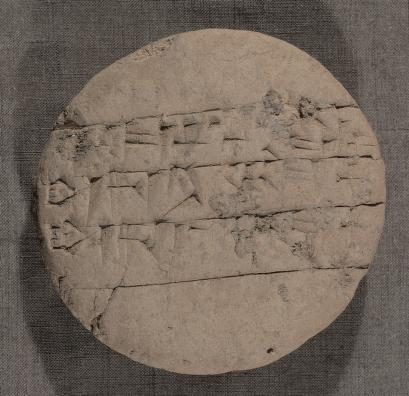
\includegraphics[width=0.3\paperwidth]{graphics/tablet01}}&%
\strut\uncover<5->{\tightbox{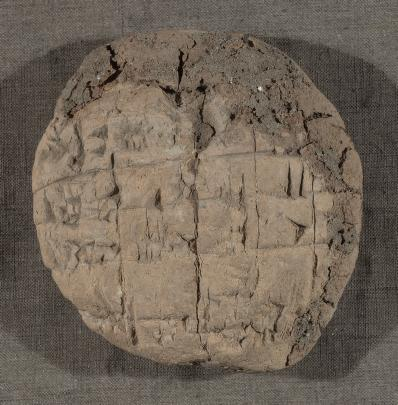
\includegraphics[width=0.3\paperwidth]{graphics/tablet02}}}&%
\strut\uncover<6->{\tightbox{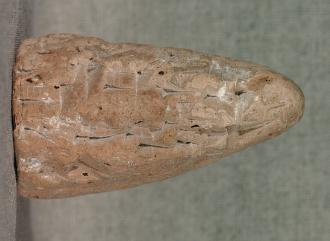
\includegraphics[height=0.3\paperwidth,angle=90]{graphics/tablet03}}}&%
\strut\uncover<7->{\tightbox{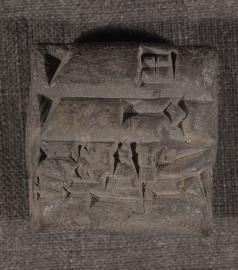
\includegraphics[height=0.3\paperwidth]{graphics/tablet04}}}&%
\strut\uncover<8->{\tightbox{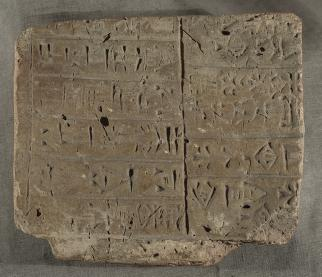
\includegraphics[height=0.3\paperwidth,angle=90]{graphics/tablet05}}}\\%
%
Sumerische Schulübung, Cuneiform tablet no.~10. Zwischen 2200 und 1900~\acrshort{BCE} \href{https://www.loc.gov/item/2020741379}{LCCN2020741379}.&%
%
\strut\uncover<5->{Altbabylonisches Kassenbuch über Fische, Cuneiform tablet no.~20. Zwischen 2200 und 1900~\acrshort{BCE} \href{https://www.loc.gov/item/2020741389}{LCCN2020741389}.}&%
%
\strut\uncover<6->{Sumerische Kegelinschrift, Cuneiform tablet no.~22. Zwischen 2200 und 1900~\acrshort{BCE} \href{https://www.loc.gov/item/2020741391}{LCCN2020741391}.}&%
%
\strut\uncover<7->{Sumerische Verkaufsrechnung, Cuneiform tablet no.~23. 2038~\acrshort{BCE} \href{https://www.loc.gov/item/2020741392}{LCCN2020741392}.}&%
%
\strut\uncover<8->{Sumerische Weiheinschrift, Cuneiform tablet no.~25. Zwischen 2144 und 2124~\acrshort{BCE} \href{https://www.loc.gov/item/2020741394}{LCCN2020741394}.}%
%
\end{tabular}}}\\%
\footnotesize{Lehmtäfelchen aus der Sammlung \citetitle{LOCCTFTROGOLTSI}\cite{LOCCTFTROGOLTSI}.}%
}}{0.03}{0.38}%
%
\end{frame}%
%
\begin{frame}%
\frametitle{Drei Aspekte der Datenhaltung}%
\begin{itemize}%
\item Wie können wir Informationen speichern?%
\item Wie können wir einen bestimmten Datensatz finden?%
\item Wie können wir representative Informationen aus unseren Daten extrahieren?%
\end{itemize}%
\end{frame}%
%
\begin{frame}%
\frametitle{Organisation von Daten}%
\uncover<-1>{%
\begin{itemize}%
\item Ein Beispiel für die Organisation von Daten ist das Dewey-System zur Organisation von Büchern in Bibliotheken, das aus den 1870ern stammt\cite{CM2003DDCPAA,OCLC2019ITTDDC}.%
\end{itemize}%
}%
\locateGraphic[Eine Illustration des Melvil Decimal Systems\cite{L2025MMDS}.]{2}{width=0.75\paperwidth}{graphics/mds}{0.125}{0.085}%
\end{frame}%
%
\begin{frame}%
\frametitle{Lochkarten}%
\uncover<-4>{%
\begin{itemize}%
\item Nicht viel später gab es die ersten Maschinen zur Datenverarbeitung.%
\item<2-> Daten wurden dabei mit physischen Werkzeugen gespeichert\cite{H1997SATAPCS1}.%
\item<3-> Das Lochkartensystem von \citeauthor{H1884AFCS}, patentiert in den späten 1880ern\cite{H1884AFCS,H1892MFTS}, wurde in der US~Volkszählung in den 1890ern verwendet.%
\item<4-> Die automatische Verarbeitung der Lochkarten erlaubte es, die Volkszählung schneller und billiger als geplant zu beenden\cite{ITIPCTPORTTIAOHMOTWD}.%
\end{itemize}%
}%
%
\locateGraphic[Skizzen von \citeauthor{H1892MFTS}'s Tabulator Machine aus dem Patent von \citeyear{H1892MFTS}\cite{H1892MFTS}.]{5}{width=0.9\paperwidth}{graphics/hollerithMachine}{0.05}{0.12}%
\end{frame}%
%
\section{Frühe Computer}%
%
\begin{frame}[t]%
\frametitle{Lochkarten 2}%
\begin{itemize}%
\item \citeauthor{H1884AFCS}'s Tabulating Machine Company fusionierte mit drei anderen Firmen zu International Business Machines~(IBM).%
\item<2-> Lochkarten waren bis in die 1950er für bis zu 20\% der Einnahmen von IBM verantwortlich\cite{ITIPCTPORTTIAOHMOTWD}.%
\end{itemize}%
%
\locateGraphic[Quelle:~\bracketCite{T2018TI0CP}~\href{https://creativecommons.org/licenses/by-sa/4.0}{CC~BY\nobreakdashes-SA~4.0}]{}{width=0.7\paperwidth}{graphics/ibm029punchedCard}{0.15}{0.38}%
\end{frame}%
%
\begin{frame}%
\frametitle{Datenorganisation}%
\begin{itemize}%
\item Neben Lochkarten gabe es noch Lochstreifen und später Magnetbänder.%
\item<2-> Die Art, wie man Daten wiederfindet, hängt davon ab, wie sie gespeichert sind.%
\item<3-> Lochkarten kann man clever sortieren und stapeln, um Informationen schnell wiederzufinden.%
\item<4-> Band-basierte Speicher müssen sequenziel vor- und zurückgespult werden.%
\item<5-> Die effiziente Organisation von Daten wurde immer wichtiger.%
\item<6-> 1958 wurde das Electronic Recording Machine Accounting~(ERMA) Mark~1 System für das Organisieren von Bankdaten entwickelt\cite{BIF1958OARORGIALSEP}.%
\item<6-> Es hatte viele Eigenschaften von Dateisystem, wobei es tatsächlich für physische, Papier-basierte Dokumente gedacht war.%
\end{itemize}%
\end{frame}%
%
\begin{frame}[t]%
\frametitle{Random Access Disk Drives}%
\begin{itemize}%
\item 1956 kam der IBM 305 RAMAC heraus: der erste Computer mit einem Random Access Disk Drive, also einer Festplatte, bei der auf Sektoren in beliebiger Reihenfolge zugegeriffen werden kann\cite{IRTFRADDRHBUCASTSFEFSFTE}.
\item<2-> Er konnte fünf bis zehn Megabytes speichern.%
\item<3-> Von nun an musste man nicht mehr auf Daten in streng sequentieller Reihenfolge zugreifen\cite{C20245YOQ}.%
\end{itemize}%
%
\locateGraphic[Quelle:~\bracketCite{G2016I3EKMUDDFW6}~ein IBM 305 RAMAC (rechts) mit zwei IBM 250 Hard Disks (Mitte und Links).]{}{width=0.7\paperwidth}{graphics/ramac}{0.15}{0.485}%
\end{frame}%
%
\begin{frame}[t]%
\frametitle{Erste Dateisysteme}%
\begin{itemize}%
\item Die ersten Dateisysteme für Computer entstanden in den 1960ern.
\item<2-> Das Atlas System in Großbritanien hatte 1961 bereits Dateisystemfunktionen.
\end{itemize}%
%
\locate{}{\resizebox{0.74\paperwidth}{!}{%
\parbox{0.7\paperwidth}{\centering\parbox{0.7\paperwidth}{%%
\parbox{0.55\linewidth}{\centering%
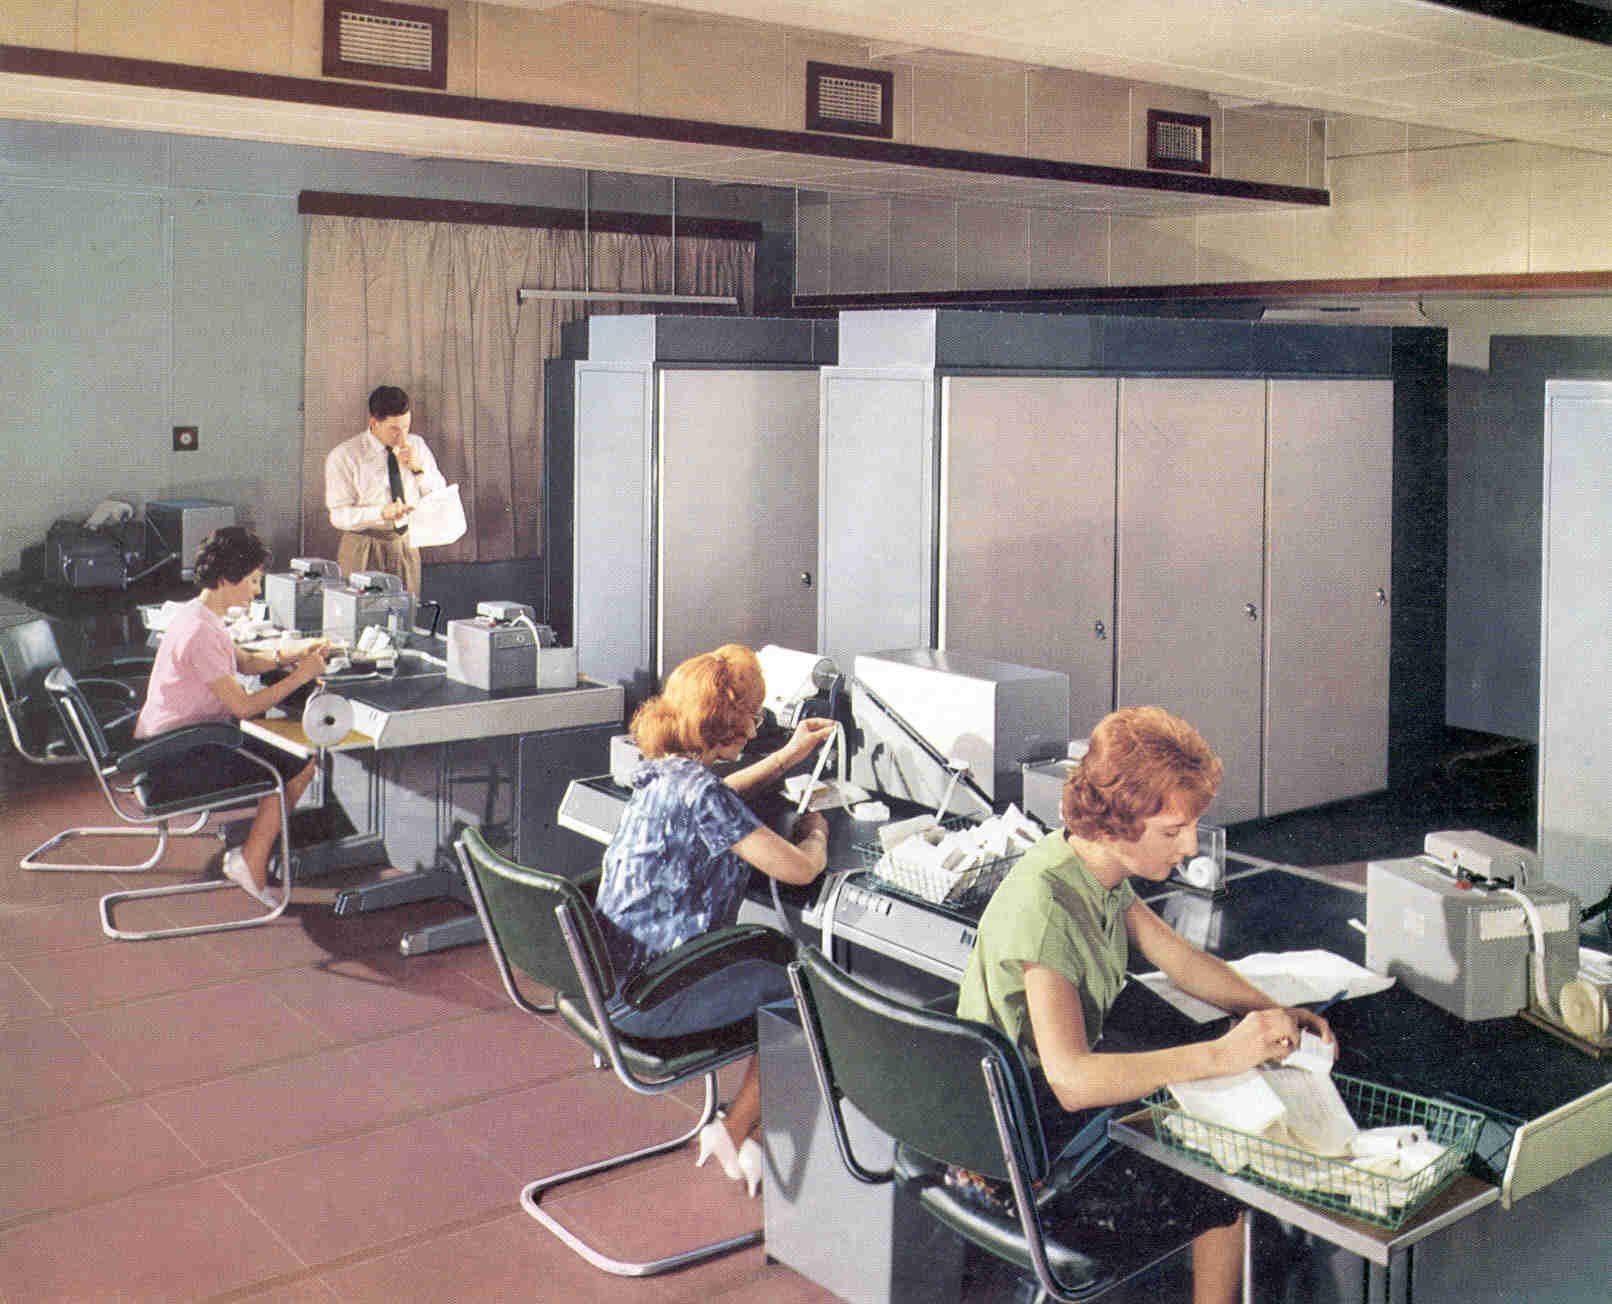
\includegraphics[width=\linewidth]{graphics/atlas3}%
}%
\strut\hfill\strut%
\parbox{0.35\linewidth}{\centering%
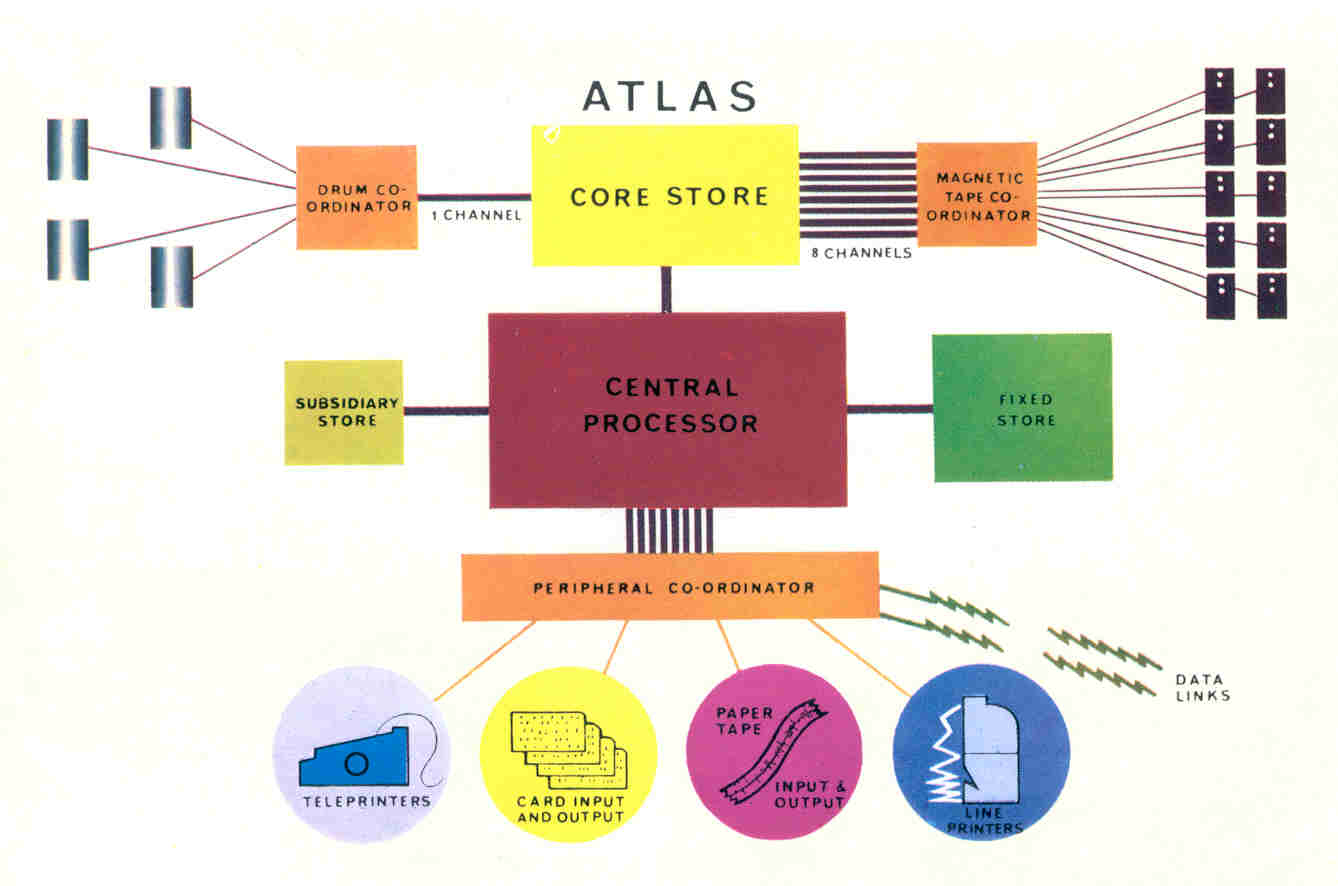
\includegraphics[width=\linewidth,trim={0 10px 0 10px},clip]{graphics/atlas1}\\[5pt]%
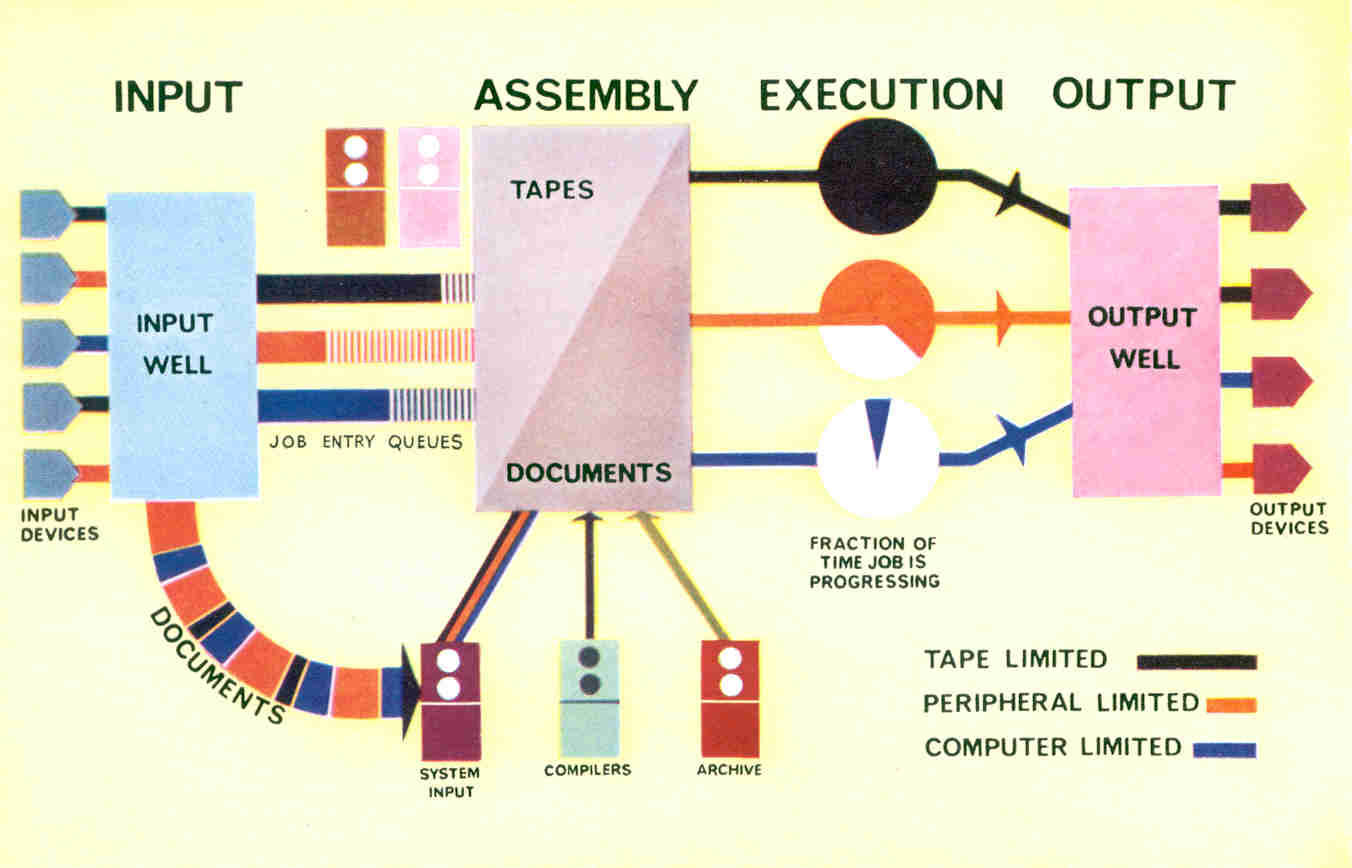
\includegraphics[width=\linewidth,trim={0 10px 0 10px},clip]{graphics/atlas2}%
}%
}\strut\\[3pt]%
\tiny{Images from the \citetitle{M2025CC:FCSA1B1}~\cite{M2025CC:FCSA1B1}. %
\textcopyright~UKRI Science and Technology Facilities Council, available from \url{https://www.chilton-computing.org.uk}.}%
}}%
}{0.13}{0.3}%
%
\end{frame}%
%
\begin{frame}[t]%
\frametitle{Erste Dateisysteme}%
\begin{itemize}%
\item 1963 hatte das Betribssystem \emph{Compatible Time-Sharing System}~(CTSS)\cite{CMDDCHOK1963TCTSSAPG} vom MIT bereits ein flaches Dateisystem ohne Ordner\cite{OD1963TCCSLABTCDE}.%
\item<2-> Das hierarchische Dateisystem des Betriebssystems \emph{Multiplexed Information and Computing Service}~(Multics)\cite{CV1965IAOOTMS,BWAOEOSH:M} hatte \citeyear{DN1965AGPFSFSS} bereits viele fortschrittliche Features die wir von heutigen Dateisystemen kennen: feingranulare Zugriffskontrolle für Datensicherheit, Backups, Links, und IO-Warteschlangen.%
\item<3-> Dateisysteme sind sehr gut zum Organisieren von Dokumenten und verschiedenartigen Daten.%
\item<4-> Sie sind jedoch nicht geeignet, um relationale Daten zu speichern und die Anforderungen an ein DBMS zu erfüllen.%
\end{itemize}%
%
\locate{-2}{\resizebox{0.95\paperwidth}{!}{%
\parbox{0.95\paperwidth}{\centering\parbox{0.95\paperwidth}{%%
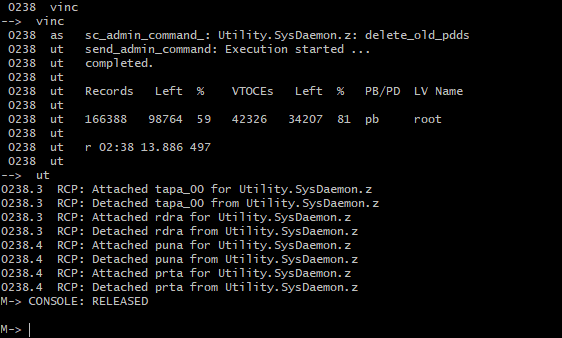
\includegraphics[width=0.32\linewidth]{graphics/multicsOperatorConsole}%
\strut\hfill\strut%
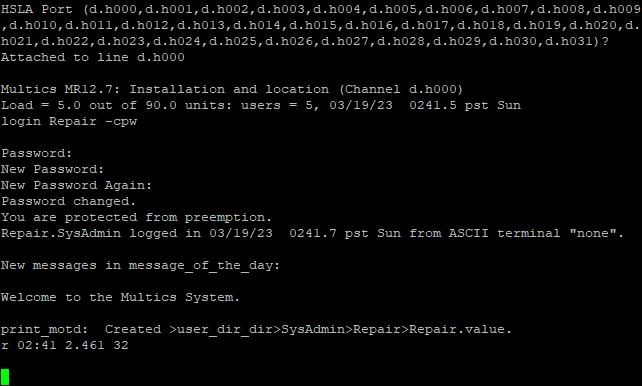
\includegraphics[width=0.32\linewidth]{graphics/multicsFirstBoot}%
\strut\hfill\strut%
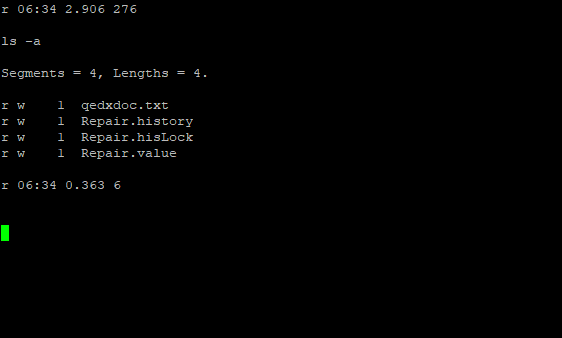
\includegraphics[width=0.32\linewidth]{graphics/multicsLs}%
}\strut\\[3pt]%
\tiny{Screenshots der Multics~MR12.7 console von~\bracketCite{BWAOEOSH:M}, \href{https://creativecommons.org/licenses/by-sa/4.0}{CC~BY\nobreakdashes-SA~4.0}.}%
}}%
}{0.025}{0.52}%
%
\end{frame}%
%
\section{Frühe Datenbanken}%
%
\begin{frame}%
\frametitle{Frühe Datenbanken}%
\begin{itemize}%
\item Es wurde klar, dass man Systeme braucht, die den Anforderungen an die Datenhaltung genügen.%
\item<2-> Aber wie sollte das gehen?%
\item<3-> Verschiedene Teams begannen, sich Ideen und Konzepte auszudenken und Prototypen zu entwickeln.%
\end{itemize}%
\end{frame}%
%
\begin{frame}%
\frametitle{Integrated Data Store}%
\begin{itemize}%
\item Die erste Version des Integrated Data Store~(IDS) wurde 1961/62 von \citeauthor{B2009TOOTIDSITFDAD} in General Electric entwickelt\cite{B2009TOOTIDSITFDAD,B1965SFRAP}.%
\item<2-> IDS war die erste Direktzugriffsdatenbank und hielt Daten im virtuellen Speicher.%
\item<3-> Es war vielleicht sogar das erste echte DBMS überhaupt.%
\item<4-> \Citeauthor{B2009TOOTIDSITFDAD} hat für seine Arbeit den 1973~A.M.~Turing Award gewonnen\cite{H2016HCBITDAFOODW}.%
\end{itemize}%
\end{frame}%
%
\begin{frame}%
\frametitle{IDS, CODASYL, und COBOL}%
\begin{itemize}%
\item IDS strukturiert Daten als ein Netzwerk und kann so komplexe Beziehungen abbilden.%
\item<2-> Der Programmierer agierte als ein Navigator durch die Daten.%
\item<3-> Die Idee war, sich Schritt-für-Schritt durch das Netz aus verknüpften Daten zu hangeln und die Daten dabei gegebenenfalls zu ändern.%
\item<4-> Dieses Netzwerkdatenmodel ist jedoch wesentlich komplexer und auch langsamer als das heute relationale Datenmodell.%
\item<5-> IDS war also nicht so flexibel.%
\item<6-> Die Database Task Group der Conference on Data Systems Languages~(CODASYL)\cite{TF1976CDBMS} war eine Standardisierungsgruppe der datenverarbeitenden Industry und übernahm \citeauthor{B2009TOOTIDSITFDAD}'s Ideen hinter dem IDS in den 1960ern.%
\item<7-> CODASYL ist heute besonders für die Entwicklung der Programmiersprache COBOL bekannt\cite{H2016HCBITDAFOODW}.%
\end{itemize}%
\end{frame}%
%
\begin{frame}%
\frametitle{Information Management System}%
\begin{itemize}%
\item Kurz nach IDS kam ein anderes System auf den Markt, das ebenfalls struturierte Daten speichern konnte.%
\item<2-> IBM entwickelte das Information Management System~(IMS) für das Apollo Space Program\cite{KLBGNLWBS2012ITIYCGTIIMS}.%
\item<3-> Das System wurde ab 1965/1967 produktiv genutzt\cite{BBP2007TBOI}.%
\item<4-> IMS existiert heute noch als Produkt und wird in einer neueren Version immer noch verkauft.%
\end{itemize}%
\end{frame}%
%
\begin{frame}%
\frametitle{Information Management System}%
\begin{itemize}%
\item Wie IDS ist auch das IMS kein relationales Datenbankmanagementsystem.%
\item<2-> Es bot stattdessen hierarchisch strukturierte Datensätze an.%
\item<3-> Ebenso wie das Netzwerkdatenmodell hat das hierarchische Datenmodell einige Nachteile\cite{KC2024DS:ITD}\uncover<4->{:%
\begin{itemize}%
\item Wenn Daten nicht streng hierarchisch strukturiert sind, dann müssen bestimmte Datensätze mehrfach gespeichert werden.%
\item<5-> In einer Datenbank in der Studenten zu Kursen zugeordnet werden, müssten alle Daten einer Studentin in jedem Datensatz jedes Kurses, den sie besucht, gespeichert werden.%
\item<6-> Die Programmiersprache, die das IMS zur Verfügung stellt, um den Datenzugriff zu implementieren, ist auch eher low-level.%
\item<7-> So muss zum Beispiel die Strategie, mit der bestimmte Daten gesucht werden, selbst implementiert werden.%
\item<8-> Und wenn sich das logische Schema der Datenbank ändert, dann führt das zu kaskadierenden Änderungen am Kode der auf die Daten zugreift.%
\end{itemize}}%
\end{itemize}%
\end{frame}%
%
\begin{frame}%
\frametitle{Der Beitrag der Ersten Datenbankmanagementsysteme}%
\begin{itemize}%
\item Sowohl IDS als auch IMS haben wichtige Beiträge geleistet.%
\item<2-> Beide boten Programmiersprachen an, mit denen auf die Daten zugegriffen werden konnte.%
\item<3-> Man konnte Typen von Datensätzen definieren und ebenso wie durch die Daten navigiert werden sollte.%
\item<4-> Man musste sich nicht mehr um die effiziente physische Speicherung kümmern.%
\item<5-> Früher musste der Kode, der Daten speichert und ließt, in \emph{allen} Programmen, die auf die Daten zugriffen, implementiert werden.%
\item<6-> Nun ist er Teil des DMBS und wir können einfachere Programmiersprachen verwenden, die davon abstrahieren.%
\end{itemize}%
\end{frame}%
%
\section{Relationale Datenbanken}%
%
\begin{frame}%
\frametitle{Weitere Probleme mit den Ersten Datenbanken}%
\begin{itemize}%
\item Sowohl das Netzwerkmodell als auch das hierarchische Modell für Daten hatten verschiedene Nachteile.%
\item<2-> Sie waren entweder kompliziert oder führten zu Redundanzen.%
\item<3-> Und obwohl die dafür angebotenen, speziellen Programmiersprachen davon abstrahierten, wie die Daten genau auf der Festplatte gespeichert werden, musste man dennoch relativ viel von dem Layout, der Struktur, und der Größe der Daten wissen, um ein performantes System zu implementieren.%
\end{itemize}%
\end{frame}%
%
\begin{frame}%
\frametitle{Weitere Probleme mit den Ersten Datenbanken}%
%
\cquotation{C1970ARMODFLSDB}{Future users of large data banks must be protected from having to know how the data is organized in the machine~(the internal representation).}%
%
\uncover<2->{%
\begin{itemize}%
\item \citeyear{C1970ARMODFLSDB} erschien das wegweisende Paper \emph{\citetitle{C1970ARMODFLSDB}} von \citeauthor{C1970ARMODFLSDB}.%
\item<3-> \Citeauthor{C1970ARMODFLSDB} hatte die Probleme des IDS-Modells erkannt, nämlich, dass Benutzer immer noch wissen mussten, wie die Daten intern organisiert werden.
\item<4-> Selbst \citeauthor{B2009TOOTIDSITFDAD} selbst hat dieses Problem mit IDS erkannt und von einem Fall berichtet, in dem die Performanz eines Systems einbrach, weil die Benutzer nicht verstanden, wie die Daten intern sortiert werden\cite{B2009TOOTIDSITFDAD}.%
\end{itemize}%
}%
\end{frame}%
%
\begin{frame}%
\frametitle{Relationale Datenbanken}%
\begin{itemize}%
\item \Citeauthor{C1970ARMODFLSDB} wollte Programmierer vor solchen Problemen schützen.%
\item<2-> Er modelliert Daten aus der \emph{relationalen} Sicht und nutzt dafür Tabellen, die er \emph{Relationen} nennt.%
\item<3-> Jede Spalte hat einen Datentyp der die zulässigen Werte definitiert.%
\item<4-> Jede Zeile muss einzigartig sein.%
\item<5-> Eine Menge von Spalten (normalerweise eine einzige spalte) bildet den Primärschlüssel, der jede Zeile eindeutig identifiziert.%
\item<6-> Zeilen in einer Tabelle können Zeilen in einer anderen Tabelle referenzieren.%
\item<7-> Dafür speichern passende Spalten der Tabelle den Primärschlüssel der anderen Tabelle als Fremdschlüssel.%
\item<8-> Daten sind nun eine Kollektion von Tabellen.%
\end{itemize}%
\end{frame}%
%
\begin{frame}%
\frametitle{Relationale Datenbanken}%
\begin{itemize}%
\item Dieses relationale Datenmodell ist einfach und besser zu implementieren.%
\item<2-> Ende der 1970ern implementieren schon mehr als ein Duzend Datenbankmanagementsysteme diese Konzepte\cite{K1979RDS}.%
\item<3-> \Citeauthor{C1970ARMODFLSDB} gewinnt dafür den A.M.~Turing Award.%
\end{itemize}%
\end{frame}%
%
\section{Datenbankzugriff über das Netzwerk}%
%
\begin{frame}%
\frametitle{Computernetzwerke}%
\begin{itemize}%
\item Der semantische Trennung von der logischen Struktur der Daten und ihrer physischen Speicherung sollte nun auch eine echte physische Trennung folgen.%
\item<2-> Computernetzwerke als verteilte Systeme entstanden in den 1960ern\cite{KR2020CNATDA}.%
\item<3-> \Citeauthor{B1960OADCACSC} hatte \citeyear{B1960OADCACSC} die Idee, Nachrichten über mehrere Netzwerkswitches zu routen\cite{B1964ODCIITDCN,B1964ODCVHAAAC,B1965ABOTDAMBN,B1960OADCACSC,B1962ODCN}.%
\item<4-> \Citeauthor{K1961IFILCNPTP} schlug \citeyear{K1961IFILCNPTP} die Idee von Paketvermittlungsnetzen vor, bei denen Nachrichten in mehrere Pakete geteilt wurden, die jeweils individuell geroutet werden, wodurch mehrere Nutzer die gleichen Netzwerkverbindungen nutzen konnten\cite{K1961IFILCNPTP}.%
\item<5-> \Citeauthor{B1962ODCN}\cite{B1962ODCN} und \Citeauthor{D1965ROLDPAICN}\cite{D1965ROLDPAICN,D1965PFTDOANCSFOLDP,D1966PFADCN} hatten ähnliche Ideen.%
\end{itemize}%
\end{frame}%
%
\begin{frame}[t]%
\frametitle{Computernetzwerke}%
\begin{itemize}\only<-2>{%
\item \Citeauthor{L1963MFMAAOTICN} \citeyear{L1963MFMAAOTICN} schlug vor, Computer- und Netzwerksprachen zu vereinheitlichen, so dass Forscher gegenseitig auf ihren Arbeiten aufbauen konnten -- der erste Schritt Richtung Internet war getan\cite{L1963MFMAAOTICN}.%
\item<2-> 1965/66 wurden der TX\nobreakdashes-2 am MIT Lincoln Lab in Massachusetts mit dem Q\nobreakdashes-32 in Santa Monica, California verbunden -- das erste Wide-Area Network war geboren\cite{L1986TAACN}.}%
\item<3-> 1967 wurde das Konzept des ARPANETs, dem Vorgänger des Internets, von der Advanced Research Projects Agency als ein Netzwerk aus 35~Computers an 16~Orten in den USA erdacht~\cite{L1986TAACN,KR2020CNATDA}.
\item<4-> 1969 waren die ersten 4~Knoten online und 1972 wurde das ARPANET öffentlich vorgestellt\cite{L1986TAACN,KR2020CNATDA}.
\end{itemize}%
%
\locateGraphic[19~Knoten Beispiel für das ARPANET, das 1968 an Hersteller verschickt wurde\cite{K2010AEHOTIHOC}]{3-}{width=0.7\paperwidth}{graphics/arpanetRFQ1968}{0.15}{0.4}%
%
\end{frame}%
%
\begin{frame}%
\frametitle{Computernetzwerke}%
\begin{itemize}%
\item \Citeauthor{CHIRW1974ABECFDBM} schlugen \citeyear{CHIRW1974ABECFDBM} vor, ein Datenbankmanagementsystem auf einem speziell dafür eingerichteten Computer laufen zu lassen\cite{CHIRW1974ABECFDBM}.%
\item<2-> Programme und Benutzer würden dann von anderen Computern über eine Netzwerkverbindung zugreifen.%
\item<3-> Das erste Ethernet wurde dann 1976 im Xerox Palo Alto Research Center~(PARC) von Metcalfe and Boggs entwickelt\cite{CHM1996CLN}.%
\item<4-> TCP/IP wird seit 1983 eingesetzt.%
\item<5-> In den 1990ern begann das Internet explosiv zu wachsen\cite{KR2020CNATDA}.%
\item<6-> Der Term \inQuotes{Client} entstand \citeyear{IMS1978SDFFIADFS} durch~\citeauthor{IMS1978SDFFIADFS}\cite{IMS1978SDFFIADFS}.%
\item<7-> Heutige Datenbankmanagementsysteme sind oftmals in der Client-Server Architektur für den Zugriff über das Netzwerk implementiert\cite{RCKS2019PNP,B1996CSA,OHE1999CSSG,RF2020FOSAAEA,EOEBEB:CSA}.%
\end{itemize}%
\end{frame}%
%
\section{Abstractions}%
%
\begin{frame}[fragile,t]
\frametitle{SQL}%
\begin{itemize}%
\item Ein weiterer wichtiger Schritt war die Sprache SEQUEL, die \citeauthor{CB1974SASEQL} \citeyear{CB1974SASEQL} als Teil des IBM System~R Projekts entwickelten\cite{CB1974SASEQL}.%
\item<2-> Die Sprache war für \citeauthor{C1970ARMODFLSDB}'s relational algebra entwickelt worden, und ermöglichte Datenbankanfragen in einer einfach verständlichen Syntax zu formulieren.%
\item<3-> Zwei Jahre später wurden Methoden zum Einfügen, Löschen, und Ändern von Datensätzen hinzugefügt\cite{CAEGLMRB1976S2AUATDDMAC}.%
\item<4-> 1977 wurde SEQUEL zu \glsreset{SQL}\sql\ abgekürzt\cite{C20245YOQ}.%
\end{itemize}%
%
\locateListingBox{5}{%
\lstinputlisting[style=sql_style,showspaces=False]{graphics/example.sql}%
}{0.05}{0.7}{0.9}{0.4}
%
\end{frame}
%
\begin{frame}%
\frametitle{Entity Relationship Diagrams}%
\begin{itemize}%
\item Bessere Abstraktionen und Werkzeuge für das Design von (relationalen) Datenbanken enstanden ebenfalls.%
\item<2-> \glsreset{ERD}\Pglspl{ERD} sind Diagramme mit denen wir die Beziehungen zwischen verschiedenen Objekten für eine Datenbank modellieren können\cite{KW2012ASHOTEDAIM,C1976TERMTAUVOD}.%
\item<3-> Sie wurden 1975 von \citeauthor{C1975TRMTAUVOD}\cite{C1975TRMTAUVOD} erfunden und wurden ein US~ANSI Standard in den späten 1980ern\cite{GK1985ATOOTIRDS,P1992IAX1ASFIRDSI}.%
\item<4-> Dabei baute \citeauthor{C1975TRMTAUVOD} auf den Datenstrukturdiarammen von \citeauthor{B1969DSD}\cite{B1969DSD} auf.%
\item<5-> \Citeauthor{C1975TRMTAUVOD} wurde auch von dem Erbe seiner Chinesischen Kultur inspiriert\cite{C1997ECAED,C2002ERMHEFTALL}.%
\end{itemize}%
%
\uncover<5>{%
\cquotation{C1997ECAED}{%
What does the Chinese character construction principles have to do with ER~modeling? %
The answer is: %
both Chinese characters and the ER~model are trying to model the world -- trying to use graphics to represent the entities in the real world. Therefore, there should be some similarities in their constructs.%
}}%
%
\locateGraphic{6}{width=0.9\paperwidth}{graphics/simpleERDexample}{0.05}{0.62}%
%
\end{frame}%
%
\section{Relationale Datenbanken im Mainstream}
%
%
\begin{frame}%
\frametitle{Computernetzwerke}%
\begin{itemize}%
\item Die Oracle Datenbank wurde als erstes kommerzielle \sql-basiertes Produkt 1979 von den Software Development Laboratories~(SDL) verkauft, die sich später in Oracle umbenannten\cite{C20245YOQ}.%
\item<2-> Sie war sofort ein Erfolg, denn sie war portierbar und konnte auf billiger Hardware laufen.%
\item<3-> IBM brachte sein \sql\ Datenbankmanagementsystem DB2 in 1983 heraus\cite{C20245YOQ,HS2013THAGOID}.%
\item<4-> \sql\ wurde \citeyear{ANSIX3135} ein US~ANSI standard und \citeyear{ISO90751987} ein internationaler ISO~standard\cite{ANSIX3135,ISO90751987}.%
\item<5-> Der Standard entwickelt sich stetig weiter, die letzte Version ist von \citeyear{ISOIEC9707112023E}\cite{ISOIEC9707112023E}.%
\item<6-> In den 1990ern, enstanden viele kostenlose Open-Source-Datenbankmanagementsysteme\cite{C20245YOQ}.%
\end{itemize}%
\end{frame}%
%
\section{Zusammenfassung}%
%
\begin{frame}%
\frametitle{Zusammenfassung}%
\begin{itemize}%
\item Seit tausenden von Jahren beschäftigen wir uns mit Datenhaltung.%
\item<2-> Seit etwa 150 Jahren nutzen wir dafür Maschinen.%
\item<3-> Seit etwa 70 Jahren haben wir Computer, auf denen Daten in sinnvollem Umfang und zu sinnvollen Kosten gespeichert werden können.%
\item<4-> Datenbanken und Computernetzwerke gibt es seit 60 Jahren.%
\item<5-> Seit 50 Jahren gibt es das Konzept der relationalen Datenbanken, die wir in diesem Kurs behandeln.%
\item<6-> Seit 30 Jahren gibt es Open Source Datenbankmanagementsysteme, wie diejenigen, die wir hier behandeln werden.%
\item<7-> Heute stehen Datenbanken hinter nahezu allen Geschäftsprozessen und liefern die Daten für die Planung für öffentliche Dienste wie das Gesundheitswesen und den öffentlicher Verkehr.%
\item<8-> Lassen Sie uns dieses Thema erforschen!%
\end{itemize}%
\end{frame}%
%
\endPresentation%
\end{document}%%
\endinput%
%
